\section[Some Special Functions]{\hyperlink{toc}{Some Special Functions}}

\subsection{Power Series, Revisited}
Recall our definition of power series (Definition \ref{def:3.38}), functions of the form:
\begin{align*}
    f(x) = \sum_{n=0}^\infty c_n x^n.
\end{align*}
Also recall the radius of convergence (Theorem \ref{thm:3.39}) of such power series, defined as:
\begin{align*}
    R = \frac{1}{\limsup_{n \rightarrow \infty}\sqrt[n]{\abs{c_n}}}.
\end{align*}
Note that if $\limsup_{n \rightarrow \infty}\sqrt[n]{\abs{c_n}} = \infty$, then $R = 0$, and if $\limsup_{n \rightarrow \infty}\sqrt[n]{\abs{c_n}} = 0$, then $R = \infty$. The series converges absolutely for $\abs{x} < R$ and diverges for $\abs{x} > R$.

\begin{figure}[htbp]
    \centering
    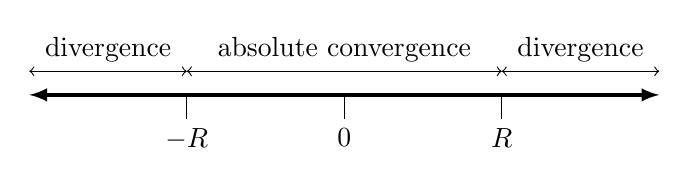
\begin{tikzpicture}[scale=2]
        \draw[latex-latex, very thick] (-2, 0) -- (2, 0);
        \draw[] (0, 0) -- (0, -0.15);
        \draw[] (1, 0) -- (1, -0.15);
        \draw[] (-1, 0) -- (-1, -0.15);
        \node[below] at (0, -0.15) {$0$};
        \node[below] at (1, -0.15) {$R$};
        \node[below] at (-1, -0.15) {$-R$};
        \draw[<->] (1, 0.15) -- (-1, 0.15);
        \draw[<->] (1, 0.15) -- (2, 0.15);
        \draw[<->] (-1, 0.15) -- (-2, 0.15);
        \node[above] at (0, 0.15) {absolute convergence};
        \node[above] at (1.5, 0.15) {divergence};
        \node[above] at (-1.5, 0.15) {divergence};
    \end{tikzpicture}
    
    \caption{Visualization of the radius of convergence for $f(x) = \sum_{n=0}^\infty c_nx^n$, $x \in \RR$.}
    \label{fig49}
\end{figure}

\begin{theorem}{}{8.1}
    If $\sum_{n=0}^\infty c_nx^n$ converges for $\abs{x} < R$, let $f(x) = \sum_{n=0}^\infty c_n x^n$ for $\abs{x} < R$. Then, the series converges uniformly on $[-R + \e, R - \e]$ for any $\e > 0$, $f$ is differentiable (and hence continuous) on $(-R, R)$ and $f'(x) = \sum_{n=0}^\infty nc_nx^{n-1}$. 
\end{theorem}

\begin{nproof}
    We first show the uniform convergence on $[-R + \e, R - \e]$. For $\abs{x} \leq R - \e$, we have that $\abs{c_nx^n} \leq \abs{x_n}(R - \e)^n$. Since $\sum_n \abs{c_n}(R - \e)^n < \infty$ (by the assumed absolute convergence on $(-R, R)$), we have that $\sum_n c_nx^n$ converges uniformly in $\abs{x} \leq R - \e$ by the M-test (Theorem \ref{thm:7.10}).

    We next prove the claim about the differentiability/derivative of $f$. The radius of convergence of $\sum_n nc_n x^{n-1}$ is:
    \begin{align*}
        \frac{1}{\limsup_{n \rightarrow \infty}\sqrt[n]{\abs{nc_n}}} = \frac{1}{\limsup_{n \rightarrow \infty}\sqrt[n]{\abs{c_n}}} = R
    \end{align*}
    so since $f$ converges in $(-R, R)$, so does $\sum_n nc_nx^{n-1}$. Now, let $s_n(x) = \sum_{m=0}^n c_mx^m$. Then, by the linearity of the derivative we have that $s_n'(x) = \sum_{m=1}^n mc_mx^{m-1}$. By the first part of the proof, we have that $s_n'(x) \rightarrow \sum_{m=1}^\infty mc_mx^{m-1}$ uniformly on $[-R + \e, R - \e]$. Since $s_n(x) \rightarrow f(x)$ uniformly, by Theorem \ref{thm:7.17}, we have that $f'$ exists on $[-R +\e, R - \e]$ and $f'(x) = \sum_{m=1}^\infty mc_mx^{m-1}$. Since $\e$ is arbitrary, $f'$ exists and is equal to $\sum_{m=1}^\infty mc_mx^{m-1}$ for all $x \in (-R, R)$. \qed 
\end{nproof}
\noindent As a remark, note that we can (interestingly) prove the differentiability of $f$ on $(-R, R)$ from the uniform convergence on $[-R + \e, R - \e]$.

\begin{ncorollary}{}{}
    If $f(x) = \sum_{n=0}^\infty c_nx^n$ converges for $\abs{x} < R$, then $f^{(k)}(x)$ exists for all $k \in \NN$ and for all $x \in (-R, R)$. It is given by:
    \begin{align*}
        f^{(k)}(x) = \sum_{n=k}^\infty n(n-1)\ldots(n-k+1)c_nx^{n-k} \quad (*)
    \end{align*}
    and consequently, we have that $c_k = \frac{f^{(k)(0)}}{k!}$, so $f(x) = \sum_{n=0}^\infty \frac{f^{(n)}(0)}{n!}x^n$.
\end{ncorollary}
\noindent Compare the above Corollary to Taylor's theorem (Theorem \ref{thm:5.15}). Here, we take our taylor polynomial and extend it to an infinite series (the limit of polynomials). 

\begin{nproof}
    By Theorem \ref{thm:8.1}, we have that $f'(x) = \sum_{n=1}^\infty nc_nx^{n-1}$ and $f''(x) = \sum_{n=2}^\infty n(n-1)c_nx^{n-2}$ and so on. Setting $x = 0$ in $(*)$, we have that $f^{(k)}(0) = n(n-1)\ldots 1 c_n = n! c_k$, so $c_n = \frac{f^{(k)}(0)}{n!}$. \qed
\end{nproof}
\noindent Recall the definition of \emph{analytic functions}, which are infinite differentiable and can be represented as sums or series of derivatives evaluated at zero. 

\begin{nexample}{}{}
    As we discussed in Chapter 5, there are infinitely differentiable functions that are not analytic. Let:
    \begin{align*}
        f(x) = \begin{cases}
            \exp(-\frac{1}{x^2}) & x \neq 0
            \\ 0 & x = 0
        \end{cases}
    \end{align*}
    By Theorem \ref{thm:8.1}, $f$ is infinitely differentiable, and $f^{(n)}(0) = 0$ for all $n \in \NN$. But, $f(x) \neq 0$ except at $x = 0$. Hence, $f(x) \neq \sum_{n=0}^\infty \frac{f^{(n)}(0)}{n!}x^n$ except at $x = 0$. This is true despite the fact that the RHS converges to zero for all $x \in \RR$. 
\end{nexample}

\begin{nexample}{}{}
    Bump functions are continuous, infinitely differentiable functions of compact support (it is zero outside of a compact set). For example, 
    \begin{align*}
        f(x) = \begin{cases}
            \exp(-\frac{1}{1-x^2}) & x \in (-1, 1)
            \\ 0 & \abs{x} \geq 1
        \end{cases}
    \end{align*}
    is an example of a bump function. Such functions are very useful in the study of functional analysis and PDEs.
\end{nexample}
\begin{figure}[htbp]
    \centering
    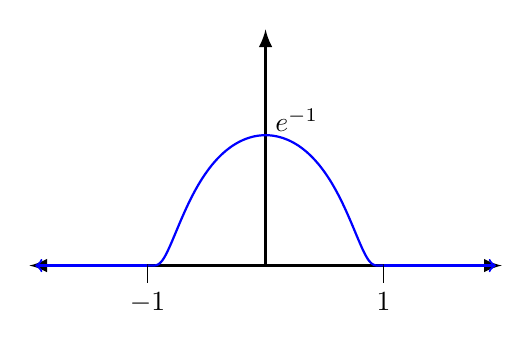
\begin{tikzpicture}[scale=1.5]
        \draw[-latex, very thick] (0, 0) -- (0, 2);
        \draw[latex-latex, very thick] (-2, 0) -- (2, 0);
        \draw[blue, thick, smooth, samples = 100, domain=-0.999:0.999, variable = \x] plot(\x, {3*exp(-1/(1-(\x)*(\x)))});
        \draw[->, blue, thick] (1, 0) -- (1.95, 0);
        \draw[->, blue, thick] (-1, 0) -- (-1.95, 0);
        \draw[] (1, 0) -- (1, -0.15);
        \draw[] (-1, 0) -- (-1, -0.15);
        \node[below] at (1, -0.15) {$1$};
        \node[below] at (-1, -0.15) {$-1$};
        \node[right] at (0, 1.23) {$e^{-1}$};
    \end{tikzpicture}
    
    \caption{Plot of the bump function $f$ from the above example.}
    \label{fig50}
\end{figure}

\noindent Before we continue, some remarks on the radius of convergence are in order. Of course, the definition of $R = \frac{1}{\limsup_{n \rightarrow \infty}\sqrt[n]{\abs{c_n}}}$ always holds. But in practice, the ratio test is much nicer to use (though it does not always work). We can make the observation that:
\begin{align*}
    \abs{\frac{c_{n+1}x^{n+1}}{c_nx^n}} = \abs{x}\abs{\frac{c_{n+1}}{c_n}} \rightarrow \abs{x}L
\end{align*}
Where we take the $n \rightarrow \infty$ limit in the final expression (assuming the limit exists). We have that the power series converges if $\abs{x} < \frac{1}{L}$ and diverges if $\abs{x} > \frac{1}{L}$. So, when the limit exists, we can write:
\begin{align*}
    R = \frac{1}{\linf\abs{\frac{c_{n+1}}{c_n}}}.
\end{align*}
In general, by Theorem 3.37 (not covered in lecture in 320, see Rudin), we have that:
\begin{align*}
    \frac{1}{\limsup_{n \rightarrow \infty}\abs{\frac{c_{n+1}}{c_n}}} \leq R \leq \frac{1}{\liminf_{n \rightarrow \infty}\abs{\frac{c_{n+1}}{c_n}}}
\end{align*}

\begin{theorem}{Abel's Theorem}{8.2}
    Suppose $\sum_{n=0}^\infty c_n$ converges (perhaps conditionally). Let $f(x) = \sum_{n=0}^\infty c_nx^n$. Then, $f(x)$ converges if $\abs{x} < 1$, and $\lim_{x \rightarrow 1^{-}}f(x) = \sum_{n=0}^\infty c_n$. 
\end{theorem}
\begin{nproof}
    For the first claim, we have that $\limsup_{n \rightarrow \infty}\sqrt[n]{\abs{c_n}} \leq 1$ so by the root test, $\sum_n c_n x^n$ has $R \geq 1$. The interesting case is when $R = 1$ (as if $R > 1$, then $f$ is continuous on $(-R, R)$ and the result follows immediately). In this case, $f(x)$ converges if $\abs{x} < 1$. Let $s_n = \sum_{m=0}^n c_m$ and $s = \sum_{m=0}^\infty c_m = \lim_{n \rightarrow \infty}s_n$. Let $s_{-1} = 0$. Then, we have that $s_n - s_{n-1} = c_n$ for $n \geq 0$.

    Let $\e > 0$. We wish to show that there exists $\delta > 0$ such that for $1 -\delta < x < 1$ we have that $\abs{f(x) - s} < \e$. We start with the partial sum of $f(x)$. For $\abs{x} < 1$, we have:
    \begin{align*}
        \sum_{m=0}^n c_mx^m &= \sum_{m=0}^n (s_m - s_{m-1})x^m
        \\ &= \sum_{m=0}^n s_mx^m - x\sum_{m=0}^{n-1}s_m x^m
        \\ &= (1-x)\sum_{m=0}^n s_mx^m + s_nx^{n+1}.
    \end{align*}
    Now, let $n \rightarrow \infty$. We then have that $s_nx^{n+1} \rightarrow 0$ as $s_n \rightarrow s$ and $x^{n+1} \rightarrow 0$. We then have that $f(x) = (1-x)\sum_{m=0}^n s_mx^m + 0$, and using that $\sum_{m=0}^\infty x^m = \frac{1}{1-x}$, we obtain that:
    \begin{align*}
        \abs{f(x) - s} = \abs{(1-x)\sum_{m=0}^\infty(s_m - s)x^m} \leq \abs{1 - x}\sum_{m=0}^\infty \abs{s_m - s}\abs{x}^m.
    \end{align*}
    Now, choose $N$ such that $m \geq N$ implies $\abs{s_m - s} < \frac{\e}{2}$. Let $x \in (0, 1)$, and then:
    \begin{align*}
        \abs{f(x) - s} \leq (1-x)\sum_{m=0}^N\abs{s_m - s}x^n + (1-x)\frac{\e}{2}\frac{1}{1-x}
    \end{align*}
    The second term on the RHS is bounded using the geometric series. The first term is a polyonimal in $x$ and hence continuous everywhere (including at $x = 1$). It equals $0$ at $x = 1$, so it has absolute value less than $\frac{\e}{2}$ if $x \in (1-\delta, 1)$ for some $\delta$. Hence:
    \begin{align*}
        \abs{f(x) - s} < \frac{\e}{2} + \frac{\e}{2} = \e
    \end{align*}
    \noindent See Rudin page 175 for an application of this Theorem to prove Theorem 3.51 in a different way. Not that for the case where $\sum_n c_n = \infty$, the theorem still holds, with $\lim_{x \rightarrow 1^-}\sum_{n=0}^\infty c_nx^n = \infty$. \qed
\end{nproof}

\begin{theorem}{}{8.3}
    Suppose $\sum_{i=1}^\infty \left(\sum_{j=1}^\infty \abs{a_{ij}}\right) < \infty$. Then, $\sum_{i=0}^\infty \sum_{j=0}^\infty a_{ij} = \sum_{j=0}^\infty \sum_{i=0}^\infty a_{ij}$ (and both converge).
\end{theorem}
\begin{nproof}
    Rudin uses an overly clever proof. See HW7Q2 for a more natural one. \qed
\end{nproof}

\begin{theorem}{}{8.4}
    Suppose $f(x) = \sum_{n=0}^\infty c_nx^n$ has radius of convergence $R$ (Taylor series of $f$ at 0/Maclaurin series). Let $\abs{a} < R$. Then, $f(x) = \sum_{n=0}^\infty \frac{f^{(n)}(0)}{n!}(x-a)^n$ for (at least) $\abs{x - a} < R - \abs{a}$. 
\end{theorem}
\begin{figure}[htbp]
    \centering
    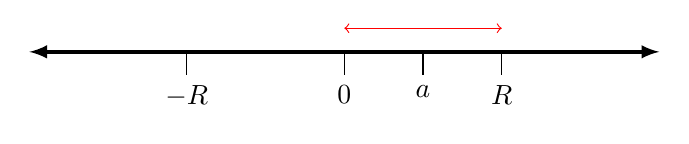
\begin{tikzpicture}[scale=2]
        \draw[latex-latex, very thick] (-2, 0) -- (2, 0);
        \draw[] (0, 0) -- (0, -0.15);
        \draw[] (1, 0) -- (1, -0.15);
        \draw[] (-1, 0) -- (-1, -0.15);
        \draw[] (0.5, 0) -- (0.5, -0.15);
        \node[below] at (0, -0.15) {$0$};
        \node[below] at (1, -0.15) {$R$};
        \node[below] at (-1, -0.15) {$-R$};
        \node[below] at (0.5, -0.15) {$a$};
        \draw[<->, red] (1, 0.15) -- (0, 0.15);
    \end{tikzpicture}
    
    \caption{Visualization of Theorem \ref{thm:8.4}. The new Taylor series around $x = a$ converges in the region up to the radius of convergence of the original series.}
    \label{fig51}
\end{figure}

\begin{nproof}
    We have that $f(x) = \sum_{n=0}^\infty c_n\left[(x - a) + a\right]^n = \sum_{n=0}^\infty c_n\sum_{m=0}^n \binom{n}{m}(x-a)^ma^{n-m}$, and we want to find a way to interchange the order of summation. By Theorem \ref{thm:8.3}, the interchange is permitted if:
    \begin{align*}
        \sum_{n=0}^\infty\sum_{m=0}^n \abs{c_n}\binom{n}{m}\abs{x-a}^m\abs{a}^{n-m} < \infty
    \end{align*}
    but the above is equaivalent to:
    \begin{align*}
        \sum_{n=0}^\infty \abs{c_n}\left(\abs{x - a} + \abs{a}\right)^n
    \end{align*}
    which converges if $\abs{x - a} + \abs{a} < R$. Therefore:
    \begin{align*}
        f(x) = \sum_{m=0}^\infty \sum_{n=m}^\infty c_n\binom{n}{m}a^{n-m}(x - a)^m
    \end{align*}
    over $n \geq m$. We need to show that these new coefficients $\left(\sum_{n=m}^\infty c_n\binom{n}{m}a^{n-m}\right)$ are equal to $\frac{f^{(m)}(a)}{m!}$. Expanding out, we have that:
    \begin{align*}
        \sum_{n=m}^\infty c_n\binom{n}{m}a^{n-m} = \frac{1}{m!}n(n-1)\ldots (n-m+1)c_na^{n-m} = \frac{1}{m!}f^{(m)}(a)
    \end{align*}
    where in the last equality we use Theorem \ref{thm:8.1}. We conclude that:
    \begin{align*}
        f(x) = \sum_{m=0}\frac{f^{(m)}(a)}{m!}(x-a)^m \text{ for } \abs{x - a} < R - \abs{a}
    \end{align*}
\end{nproof}

\begin{nexample}{}{}
    Let $f(x) = \sum_{n=0}^\infty x^n$. If $\abs{x} < 1$, then the series converges and $f(x) = \frac{1}{1-x}$ ($R = 1$). Choose $a = -\frac{1}{2}$ (we look at the Taylor serires around $x = -\frac{1}{2}$). For any $\abs{x} < 1$, we have that $f^{(n)}(x) = \frac{n!}{(1-x)^{n+1}}$, so therefore:
    \begin{align*}
        f^{(n)}(-\frac{1}{2}) = \frac{n!}{(1+\frac{1}{2})^{n+1}} = \left(\frac{2}{3}\right)^{n+1}n!.
    \end{align*}
    By Theorem \ref{thm:8.4}, we then have that:
    \begin{align*}
        f(x) = \sum_{n=0}^\infty \frac{\left(\frac{2}{3}\right)^{n+1}n!}{n!}(x - a)^n = \sum_{n=0}^\infty \left(\frac{2}{3}\right)^{n+1}(x + \frac{1}{2})^n
    \end{align*}
    which is valid for $\abs{x - (-\frac{1}{2})} < 1 - \abs{-\frac{1}{2}}$ and hence if $\abs{x + \frac{1}{2}} < \frac{1}{2}$. Note that in fact, $\sum_{n=0}^\infty\left(\frac{2}{3}\right)^{n+1}(x - a)^n$ converges whenever $\abs{\frac{2}{3}(x + \frac{1}{2})} < 1$, in other words, whenever $\abs{x + \frac{1}{2}} < \frac{3}{2}$, so the series converges in $(-\frac{3}{2}, \frac{1}{2})$. 
\end{nexample}
\begin{figure}[htbp]
    \centering
    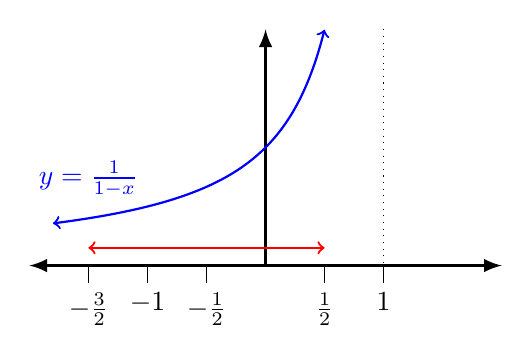
\begin{tikzpicture}[scale=1.5]
        \draw[-latex, very thick] (0, 0) -- (0, 2);
        \draw[latex-latex, very thick] (-2, 0) -- (2, 0);
        \draw[blue, thick, smooth, <->, samples = 100, domain=-1.8:0.5, variable = \x] plot(\x, {1/(1 - (\x))});
        \draw[] (1, 0) -- (1, -0.15);
        \draw[] (-1, 0) -- (-1, -0.15);
        \draw[] (-0.5, 0) -- (-0.5, -0.15);
        \draw[] (-1.5, 0) -- (-1.5, -0.15);
        \draw[] (0.5, 0) -- (0.5, -0.15);
        \node[below] at (0.5, -0.15) {$\frac{1}{2}$};
        \node[below] at (1, -0.15) {$1$};
        \node[below] at (-1, -0.15) {$-1$};
        \node[below] at (-0.5, -0.15) {$-\frac{1}{2}$};
        \node[below] at (-1.5, -0.15) {$-\frac{3}{2}$};
        \node[above, text = blue] at (-1.5, 0.5) {$y = \frac{1}{1-x}$};
        \draw[dotted] (1, 2) -- (1, -0.15);
        \draw[<->, red, thick] (-1.5, 0.15) -- (0.5, 0.15);
    \end{tikzpicture}
    
    \caption{Plot of $y = \frac{1}{1-x}$ and region for which the Taylor series around $a = -\frac{1}{2}$ is valid (red).}
    \label{fig52}
\end{figure}
\noindent As a remark, note that although Theorem \ref{thm:8.4} only guarantees convergence up to the previous boundary, in general the Taylor series will converge up to the nearest singularity. The above theorem is a good example of \emph{analytic continuation}, where a representation of a function converges in a larger interval than the original series (notice that the above taylor series for $f$ around $a = -\frac{1}{2}$ converges up to $-\frac{3}{2}$, when the original series only converged up to $-1$). We extend the function to a larger interval.

Note that there is another way to obtain the Taylor series around $a = -\frac{1}{2}$ (in a technique reminiscent of that used in MATH 300). We can cleverly manipulate the original expression and the geometric series formula to observe that:
\begin{align*}
    f(x) = \frac{1}{1 - x} = \frac{1}{1 - x + \frac{1}{2} - \frac{1}{2}} = \frac{2}{3}\frac{1}{1 - \frac{2}{3}(x + \frac{1}{2})} = \frac{2}{3}\sum_{n=0}^\infty \left(\frac{2}{3}\right)^n (x + \frac{1}{2})^n.
\end{align*}

\begin{theorem}{Principle of Permanence of Form}{8.5}
    Suppose $\sum_n a_n x^n$ and $\sum_n b_n x^n$ each have radius of convergence larger or equal to $R$. Suppose $D \subset (-R, R)$ has a limit point in $(-R, R)$ (for example, $D = \set{\frac{R}{n}: n = 2, 3, \ldots}$ with limit point $0$). If $\sum_n a_nx^n = \sum_n b_n x^n$ in all $x \in D$, then $a_n = b_n$ for all $n \in \NN$ and $\sum_n a_nx^n$ and $\sum_n b_n x^n$ for all $x \in (-R, R)$. 
\end{theorem}
\noindent Note that this also holds for complex variables, so it can be a way of taking things we know in a real context and promoting it to a complex context. We will first prove a lemma.

\begin{nlemma}{ (Problem 2.6)}{}
    Let $E \subset X$ for a metric space $X$. Then the set $E'$ of limit points of $E$ is closed.
\end{nlemma}
\begin{nproof}
    Let $x$ be a limit point of $E'$. We wish to show that $x \in E'$. Let $\delta > 0$. Since $x$ is a limit point of $E'$, for any $r > 0$ there exists some $y \in E'$, $y \neq x$ such that $y \in N_r(x)$. Since $y \in E'$, for any $\delta - r > 0$ we have that $N_{\delta-r}(y)$ contains a point $z$ of $E$. Therefore, we have that:
    \begin{align*}
        d(x, z) \leq d(x, y) + d(y, z) < r + \delta - r = \delta
    \end{align*}
    so any neighbourhood $N_\delta(x)$ of $x$ contains some point of $E$. Hence, $x$ is a limit point of $E$ and $x \in E'$. Hence $E'$ is closed. \qed
\end{nproof}
\noindent We now move to the proof of the theorem.
\begin{nproof}
    Let $c_n = a_n - b_n$ and $f(x) = \sum_n c_nx^n$. Then, $f(x) = 0$ for all $x \in D$. Let $E = \set{x \in (-R, R): f(x) = 0}$, so $D \subset E$. We want to show that $E = (-R, R)$. Let $A = E' \cap (-R, R)$. By hypothesis, $A \neq \emptyset$ as $D$ has a limit point in $(-R, R)$. Let $B = (-R, R) \setminus A$. Then, $(-R, R) = A \cup B$ and $A \cap B = \emptyset$. By the above Lemma, the set of limit points $E'$ is closed. Hence, $A$ is closed and $B$ is open. We claim that $A$ is also open.

    To see that this is the case, we show that $E'$ is open (then $E' \cap (-R, R)$ is open as a finite intersection of open sets is open). Let $x_0 \in A$. Then, there exists $d_n$ such that $f(x) = \sum_n d_n(x - x_0)^n$ for $\abs{x - x_0} < R - \abs{x_0}$ by Theorem \ref{thm:8.4}. We will show that $d_n = 0$ for all $n$, showing that $f(x) = 0$ for all $x \in I_0 = N_{R - \abs{x_0}}(x_0)$, and therefore that $A$ is open. Suppose for the sake of contradiction that this is false. Then, there exists $k$ such that $d_k \neq 0$, i.e. $f(x) = \sum_{n=k}^\infty d_n(x - x_0)^n$ with $d_k \neq 0$. So, $f(x) = (x-x_0)^k\sum_{n=0}^\infty d_{n+k}(x - x_0)^n = g(x)$. Then, $g(x_0) = d_k \neq 0$. By the continuity of $g$, there exists $\delta > 0$ such that $g(x) \neq 0$ for $\abs{x - x_0} < \delta$. But then, $f(x) = (x - x_0)^kg(x) \neq 0$ if $0 < \abs{x - x_0} < \delta$. But then we have that there exists a neighbourhood of $x_0$ such that $f(x) \neq 0$, but then $x_0$ cannot be a limit point of $\set{x: f(x) = 0}$. So, $x_0 \notin A$, which is a contradiction. Hence $d_n = 0$ for all $n \in \NN$, and $A$ is open. 
    
    Given the claim, we have that $A \cap \overline{B} = \overline{A} \cap B = \emptyset$ and hence $A$ and $B$ are separated sets. Since $(-R, R)$ is connected and equals $A \cup B$, one of $A, B$ must be empty. It cannot be $A$ (as $E' \neq \emptyset$ by assumption) so it must be $B$. Hence $B = \emptyset$ and $A = (-R, R) = E'$. This means that any $x \in (-R, R)$ is a limit point of $E$, so there exists $\set{x_n} \subset E$ such that $x_n \rightarrow x$. Since $f$ is continuous on $(-R, R)$, we have that $f(x) = \linf f(x_n) = 0$. So, $x \in E$ and $E = (-R, R)$. \qed
\end{nproof}
\noindent Having proven some more properties of power series, we now move to formal definitions of the exponential/logarithmic/trigonometric functions and a from-first-principles proof of their properties. 

\subsection{The Exponential Function}
Recall Definition \ref{def:3.30}, where we defined $e = \sum_{n=0}^\infty \frac{1}{n!}$. We also showed in Theorem \ref{thm:3.31} that $e = \linf\left(1 + \frac{1}{n}\right)^n$. We also know that $2 < e < 3$, and  by Theorem \ref{thm:3.32} that $e$ is irrational. We now define a power series based on $e$. 

\begin{ndef}{: The Exponential Function}{}
    For $z \in \CC$, we define:
    \begin{align*}
        E(z) = \sum_{n=0}^\infty \frac{z^n}{n!}
    \end{align*}
\end{ndef}
\noindent In particular, we note that $E(1) = e$. Also note that (from Example \ref{exam:3.40}) that the above power series has radius of convergence $R = \infty$. We will show with the next sequence of theorems that $E(z)$ coincides with the exponential function $\exp(z) = e^z$ that we are familiar with.

\begin{ntheorem}{: Addition Formula}{}
    For $z, w \in \CC$, we have that $E(z + w) = E(z)E(w)$.
\end{ntheorem}
\begin{nproof}
    From the defintion, we have that:
    \begin{align*}
        E(z)E(w) &= \sum_{n=0}^\infty \frac{z^n}{n!}\sum_{m=0}^\infty\frac{w^m}{m!}
        \\ &= \sum_{n=0}^\infty \sum_{k=0}^n \frac{z^k}{k!}\frac{w^{n-k}}{(n-k)!}
        \\ &= \sum_{n=0}^\infty \frac{1}{n!}\sum_{k=0}^n\binom{n}{k}z^kw^{n-k}
        \\ &= \sum_{n=0}^\infty \frac{1}{n!}(z + w)^n
        \\ &= E(z + w)
    \end{align*}
    where in the second equality we use Theorem \ref{thm:3.50} for the multiplication of series. \qed
\end{nproof}
\noindent We can now use this addition formula to show how $E(p)$ coincides with $\exp(p)$:

\begin{ntheorem}{}{}
    For $p \in \QQ, E(p) = e^p$. 
\end{ntheorem}
\begin{nproof}
    Setting $z = w = 1$ in the addition formula above, we note that:
    \begin{align*}
        E(2) = E(1 + 1) = E(1)^2 = e^2, \quad E(3) = E(2 + 1) = E(2)E(1) = e^2e^1 = e^3
    \end{align*}
    so by induction, it follows that for $n \in \NN$:
    \begin{align*}
        E(n) = e^n
    \end{align*}
    Furthermore, we observe that:
    \begin{align*}
        E(z)E(-z) = E(z - z) = E(0) = 1
    \end{align*}
    so it follows that $E(z) = \frac{1}{E(z)}$. Hence, $E(-N) = \frac{1}{e^N} = e^{-N}$ for $N \in \NN$. Finally, let $p = \frac{m}{n}$ with $m, n \in \NN$. Then, we have that:
    \begin{align*}
        e^m = E(m) = E(np) = E(p + \ldots + p) = E(p)^n
    \end{align*}
    so therefore:
    \begin{align*}
        E(\frac{m}{n}) = E(p) = e^{\frac{m}{n}}
    \end{align*}
    Additionally, we have that:
    \begin{align*}
        1 = E(p - p) = E(p)E(-p) = e^pE(-p) \implies E(-p) = \frac{1}{e^p}.
    \end{align*}
    We have hence successfully shown that $E(p) = e^p$ for $p \in \QQ$. \qed
\end{nproof}
\noindent Next, we will extend the theorem for real exponents and study properties. We will have to come up with a different definition for an exponential of irrational powers; note that so far, our definition for exponentials $a^x$ only could accomodate rational $x$. 

\begin{ndef}{: Real Exponentials}{}
    For $x \in \RR$, let:
    \begin{align*}
        e^x = E(x) = \sum_{n=0}^\infty \frac{x^n}{n!}
    \end{align*}
\end{ndef}
\noindent The above defintion defines $x \mapsto e^x$ as an analytic function on $\RR$, which is therefore infinitely differentiable on $\RR$. Futhermore, the derivatives have a certain property.
\begin{ntheorem}{}{}
    $\od{}{x}e^x = e^x$.
\end{ntheorem}
\begin{nproof}
    By the defintion of $e^x$ we have that:
    \begin{align*}
        \dod{}{x}e^x = \sum_{n=0}^\infty \dod{}{x}\left(\frac{x^n}{n!}\right) = \sum_{n=0}^\infty \left(\frac{nx^{n-1}}{(n-1)!}\right) = \sum_{n=1}^\infty \frac{x^{n-1}}{(n-1)!} = \sum_{n=0}^\infty \frac{x^n}{n!} = e^x
    \end{align*} \qed
\end{nproof}

\begin{ntheorem}{}{}
    $e^x > 0$ for all $x \in \RR$.
\end{ntheorem}
\begin{nproof}
    Since $e^{x+y} = e^xe^y$ by the addition formula, we have for any $x \in \RR$ that $e^{x}e^{-x} = 1$. Since $e^x > 0$ if $x \geq 0$ by definition, it follows that $e^{-x} > 0$ as well if $e^{x}e^{-x} = 1 > 0$ is to be satisfied. \qed
\end{nproof}

\begin{ntheorem}{}{}
    $e^x$ is strictly increasing and strictly convex.
\end{ntheorem}
\begin{nproof}
    Since $\od{}{x} e^x = e^x > 0$ and $\od[2]{}{x} e^x = e^x > 0$ by the two previous theorems, we conclude that $e^x$ is strictly increasing and convex by Theorems \ref{thm:5.11} (and its extension). \qed
\end{nproof}

\begin{ntheorem}{: Superpolynomial Asymptotic Growth}{}
    $\lim_{x \rightarrow \infty} \frac{e^x}{x^n} = \infty$.
\end{ntheorem}
\begin{nproof}
    For $n \geq 0$, the defintion shows that:
    \begin{align*}
        e^x > \frac{x^{n+1}}{(n+1)!}
    \end{align*}
    if $x > 0$, as on the RHS we drop all but the $k = n+1$ term in the series (and all of the terms are positive for $x > 0$). Rearranging, we have that:
    \begin{align*}
        \frac{e^x}{x^n} > \frac{x}{(n+1)!}
    \end{align*}
    and the claim follows by taking $x \rightarrow \infty$. \qed
\end{nproof}
\noindent The above theorem shows that $e^x$ grows faster than any power of $x$. We also obtain the Corollary:
\begin{ncorollary}{}{}
    $\lim_{x \rightarrow \infty} e^x = \infty$, $\lim_{x \rightarrow \infty} e^{-x} = 0$. 
\end{ncorollary}
\begin{nproof}
    The first claim follows by setting $n = 0$ in the previous Theorem, and the second by using that $e^{-x} = \frac{1}{e^x}$. \qed
\end{nproof}
\noindent Since $e^x$ is strictly increasing, we may now define an inverse of $e^x$ at each $y > 0$. 

\subsection{The Logarithm}
\begin{ndef}{: The Logarithm}{}
    For $y > 0$, define $L(y) = \log(y)$ by $E(L(y)) = y$ for $y > 0$, $y \in \RR$. Equivalently, we can define the logarithm as $L(E(x))) = x$ for $x \in \RR$ or $e^{\log y} = y$ or $\log e^x = x$. 
\end{ndef}
\begin{figure}[htbp]
    \centering
    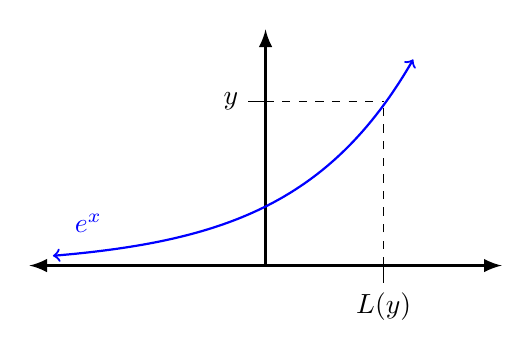
\begin{tikzpicture}[scale=1.5]
        \draw[-latex, very thick] (0, 0) -- (0, 2);
        \draw[latex-latex, very thick] (-2, 0) -- (2, 0);
        \draw[blue, thick, smooth, <->, samples = 100, domain=-1.8:1.25, variable = \x] plot(\x, {0.5*exp(\x)});
        \node[above, text = blue] at (-1.5,0.2) {$e^x$};
        \draw[dashed] (0, 1.39) -- (1, 1.39);
        \draw[dashed] (1, 0) -- (1, 1.39);
        \draw[] (0, 1.39) -- (-0.15, 1.39);
        \node[left] at (-0.15, 1.39) {$y$};
        \draw[] (1, 0) -- (1, -0.15);
        \node[below] at (1, -0.15) {$L(y)$};
    \end{tikzpicture}

    \caption{Plot of $e^x$ and extraction of its inverse $L(y)$.}
    \label{fig53}
\end{figure}

\begin{ntheorem}{: Derivative and Addition Formula}{}
    $L'(y) = \frac{1}{y}$ for $y > 0$ and $L(uv) = L(u) + L(v)$
\end{ntheorem}
\begin{nproof}
    Since $L(E(x)) = x$ by definition, by the chain rule (Theorem \ref{thm:5.5}) we have that:
    \begin{align*}
        L'(E(x))E'(x) = 1 \implies L'(E(x)) = \frac{1}{E(x)}.
    \end{align*}
    Where we use that $E'(x) = E(x)$ in the above implication. Letting $E(x) \mapsto y$, we have that $L'(y) = \frac{1}{y}$ as claimed. For the second claim, consider that for all $u, v > 0$, there exists unique $x, y \in \RR$ (which can be denoted as $\exists ! x, y \in \RR$) such that $E(x) = u, E(y) = v$. Hence:
    \begin{align*}
        L(uv) = L(E(x)E(y)) = L(E(x + y)) = x + y = L(u) + L(v).
    \end{align*}\qed
\end{nproof}

\begin{ncorollary}{}{}
    For $y > 0$, $L(y) = \int_1^y \frac{1}{t}dt$.
\end{ncorollary}
\begin{nproof}
    By the Fundamental Theorem of Calculus (Theorem \ref{thm:6.21}) we have that $\int_1^y \frac{1}{t}dt = L(y) - L(1) = L(y)$. \qed
\end{nproof}

\begin{ntheorem}{}{}
    For $p \in \QQ$, $L(x^p) = pL(x)$.
\end{ntheorem}
\begin{nproof}
    By the addition formula, we have that $L(\frac{1}{x}) + L(x) = L(\frac{1}{x}x) = L(1) = 0$. Hence, $L(\frac{1}{x}) = -L(x)$. Furthermore, by the addition formula, we have that $L(x^n) = nL(x)$ by induction. Furthermore, $L(x^0) = L(1) = 0 = 0L(x)$ which shows that the formula holds for $\NN \cup \set{0}$. Combining the previous facts, we have that:
    \begin{align*}
        nL(x^{\frac{1}{n}}) = L((x^{\frac{1}{n}})^n) = L(x^1) \implies L(x^{\frac{1}{n}}) = \frac{1}{n}L(x)
    \end{align*} 
    We therefore have that for $p = \frac{m}{n}$ with $m, n \in \NN$ that:
    
    \begin{align*}
        L(x^{\frac{m}{n}}) = mL(x^{\frac{1}{n}}) = \frac{m}{n}L(x)
    \end{align*}
    Furthermore,
    \begin{align*}
        L(x^{-\frac{m}{n}}) = L\left(\frac{1}{x^{\frac{m}{n}}}\right) = -L(x^{\frac{m}{n}}) = -\frac{m}{n}L(x)
    \end{align*}
    which shows that the proposed identity holds for all $p \in \QQ$. \qed
\end{nproof}

\begin{ndef}{: Real Exponentials with Arbitrary Base}{}
    For $\alpha \in \RR$, we define $x^\alpha = e^{\alpha \log \alpha}$.
\end{ndef}
\noindent Note that the above definition is equivalen to the definition made in MATH 320 HW3Q1, but it is a much cleaner definition (as we will soon see)!

\begin{ntheorem}{: Generalized Power Rule}{}
    $\od{}{x}x^\alpha = \alpha x^{\alpha -1}$ and hence $x^\alpha$ has antiderivative:
    \begin{align*}
        \begin{cases}
            \frac{1}{\alpha + 1}x^{\alpha + 1} & \text{if $\alpha \neq -1$}
            \\ \log x & \text{if $\alpha = 1$}
        \end{cases}.
    \end{align*}
\end{ntheorem}
\begin{nproof}
    From the definition of $x^\alpha$, we have that:
    \begin{align*}
        \dod{}{x}x^\alpha = \dod{}{x}\left(e^{\alpha \log x}\right) = e^{\alpha \log x} \alpha\frac{1}{x} = \alpha\frac{x^\alpha}{x} = \alpha x^{\alpha - 1}
    \end{align*}
    where in the second equality we use the chain rule and the fact that $L'(y) = \frac{1}{y}$. \qed
\end{nproof}

\begin{ntheorem}{: Subpolynomial Asymptotic Growth}{}
    $\lim_{x \rightarrow \infty} \log x = \infty$, $\lim_{x \rightarrow 0^+} = -\infty$, and $\lim_{x \rightarrow \infty} \frac{\log x}{x^\alpha} = 0$ if $\alpha > 0$.
\end{ntheorem}
\begin{nproof}
    To realize the first two equalities, we first make the observation that $\log(x)$ is (Strictly) monotonically increasing. To see this, let $x_1, x_2 > 0$ and $x_1 < x_2$ and then we have that:
    \begin{align*}
        \log(x_2) - \log(x_1) = \int_0^{x_2} \frac{1}{t}dt - \int_0^{x_1}\frac{1}{t}dt = \int_{x_1}^{x_2}\frac{1}{t}dt > 0
    \end{align*}
    where the bound follows from the fact that $\frac{1}{t} > 0$ for all $t > 0$ and $x_2 - x_1 > 0$. Hence, $\log(x)$ is monotonicaly increasing, and to compute the limits it suffices to compute the limit along a specific choice of sequence that tends to $\infty$ or $0$ respectively. Using that $\linf e^n = \infty$ and $\linf e^{-n} = 0$, we have that:
    \begin{align*}
        \linf \log(e^n) = \linf n\log(e) = \linf n = \infty
    \end{align*}
    \begin{align*}
        \linf \log(e^{-n}) = \linf -n\log(e) = \linf -n = -\infty
    \end{align*}
    so we conclude that $\lim_{x \rightarrow \infty}\log(x) = \infty$ and $\lim_{x \rightarrow 0} \log(x) = -\infty$.

    For the third claim, we let $a > 0$ and $x > 1$. Then:
    \begin{align*}
        \log(x) = \int_1^x \frac{1}{t}dt < \int_1^x t^a\frac{1}{t}dt = \left.\frac{t^a}{a}\right|_{1}^x = \frac{x^a}{a} - \frac{1}{a} < \frac{x^a}{a}
    \end{align*}
    so choosing $a \in (0, \alpha)$ we have that:
    \begin{align*}
        \frac{1}{x^\alpha}\log x < \frac{1}{a}\frac{1}{x^{\alpha - a}} \rightarrow 0 \text{ as } x \rightarrow \infty.
    \end{align*}\qed
\end{nproof}

\subsection{Cosine and Sine}
We have seen that $E(z+w) = E(z)E(w)$ for all $z, w \in \CC$. A natural definition for the complex exponential follows.

\begin{ndef}{: Complex Exponentials}{}
    Given $z \in \CC$, we define:
    \begin{align*}
        e^z = \sum_{n=0}^\infty \frac{z^n}{n!} = E(z)
    \end{align*}
\end{ndef}
\noindent As a remark, note in taking the complex conjugate of $\exp(z)$, we can absorb the conjugation into the argument:
\begin{align*}
    \overline{\exp(z)} = \overline{\sum_{n=0}^\infty \frac{z^n}{n!}} = \sum_{n=0}^\infty \frac{\overline{z}^n}{n!} = \exp(\overline{z})
\end{align*}
\noindent We will now define the trigonometric functions using the complex exponential, and prove the properties that we would expect them to have from our prior geometric notions.

\begin{ndef}{: Cosine and Sine}{}
    Let $x \in \R$. We then define:
    \begin{align*}
        C(x) &= \Re E(ix) = \frac{1}{2}\left[e^{ix} + e^{-ix}\right]
        \\ S(x) &= \Im E(ix) = \frac{1}{2i}\left[e^{ix} - e^{-ix}\right]
    \end{align*}
\end{ndef}

\begin{ntheorem}{: Euler's Formula}{}
    $E(ix) = C(x) + iS(x)$. 
\end{ntheorem}
\begin{nproof}
    The formula is an immediate consequence of the definitions of $C(x), S(x)$. \qed
\end{nproof}
\noindent Note that $C(x), S(x)$ can alternatively (equivalently) be defined as power series:
\begin{align*}
    C(x) &= \frac{1}{2}\sum_{n=0}^\infty \left(\frac{(ix)^n}{n!} + \frac{(-ix)^n}{n!}\right) = \sum_{n=0}^\infty (-1)^n \frac{x^{2n}}{(2n)!}
    \\ S(x) &= \sum_{n=0}^\infty (-1)^n \frac{x^{2n}}{(2n+1)!}
\end{align*}

\begin{ntheorem}{}{}
    Let $x \in \RR$. We then have that:
    \begin{enumerate}
        \item $C(x) = C(-x)$, $C(0) = 1$ and $S(x) = -S(-x)$, $S(0) = 0$.
        \item $C^2(x) + S^2(x) = 1$.
        \item $C'(x) = -S(x)$ and $S'(x) = C(x)$.
    \end{enumerate}
\end{ntheorem}

\begin{nproof}
    \begin{enumerate}
        \item From the definitions of $C$ and $S$, we have:
        \begin{align*}
            C(-x) &= \frac{1}{2}\left[e^{-ix} + e^{ix}\right] = C(x)
            \\ C(0) &= \frac{1}{2}\left[e^{i(0)} + e^{-i(0)}\right] = \frac{1}{2}\left[1 + 1\right] = 1
            \\ -S(-x) &= -\frac{1}{2}\left[e^{-ix} - e^{ix}\right] = \frac{1}{2}\left[e^{ix} - e^{-ix}\right] = S(x)
            \\ S(0) &= \frac{1}{2}\left[e^{i(0)} - e^{-i(0)}\right] = \frac{1}{2}\left[1 - 1\right] = 0
        \end{align*}
        \item Expanding out the expression, we have:
        \begin{align*}
            C^2(x) + S^2(x) &= \frac{1}{4}\left[e^{ix}e^{ix} + 2e^{ix}e^{-ix} + e^{-ix}e^{-ix}\right] - \frac{1}{4}\left[e^{ix}e^{ix} - 2e^{ix}e^{-ix} + e^{-ix}e^{-ix}\right]
            \\ &= e^{ix}e^{-ix}
            \\ &= e^{ix - ix}
            \\ &= e^0
            \\ &= 1
        \end{align*}
        \item Using the linearity of the derivative, and the known result for the derivative of exponentials we have:
        \begin{align*}
            C'(x) &= \frac{1}{2}\left[ie^{ix} - ie^{-ix}\right] = -\frac{1}{2i}\left[e^{ix} - e^{-ix}\right] = -S(x)
            \\ S'(x) &= \frac{1}{2i}\left[ie^{ix} + ie^{-ix}\right] = \frac{1}{2}\left[e^{ix} + e^{-ix}\right] = C(x)
        \end{align*} \qed
    \end{enumerate}
\end{nproof}

\begin{nlemma}{}{}
    There exists $x > 0$ such that $C(x) = 0$. 
\end{nlemma}
\begin{nproof}
    Suppose for the sake of contradiction that $C(x) > 0$ for all $x > 0$. Then, $S$ is strictly increasing as $S' = C$. So, for all $y > x$, we then have that:
    \begin{align*}
        S(x)(y - x) < \int_x^y S(t)dt = -C(y) + C(x) \leq 2
    \end{align*}
    but letting $y \rightarrow \infty$, we get that $\infty \leq 2$ which is a contradiciton. \qed
\end{nproof}

\begin{ndef}{: $\pi$}{}
    Given the above Lemma, $x_0 = \inf\set{x > 0: C(x) = 0}$ exists. In particular, $x_0 > 0$ since $C(0) = 1$ and $C$ is continuous. Then, we define $\pi = 2x_0$. 
\end{ndef}

\begin{ntheorem}{}{}
    $S(\frac{\pi}{2}) = 1$.
\end{ntheorem}
\begin{nproof}
    By the definition of $\pi$, we have that $C(x) > 0$ for $x \in [0, \frac{\pi}{2})$ and $C(\frac{\pi}{2}) = 0$. From the previous theorem we have that $C^2(\frac{\pi}{2}) + S^2(\frac{\pi}{2}) = 1$ so we obtain that $S(\frac{\pi}{2}) = \pm 1$. Since $S(0) = 0$ and $S'(x) = C(x) > 0$ for $x \in [0, \frac{\pi}{2})$, we conclude that $S(\frac{\pi}{2}) = 1$. \qed
\end{nproof}
\noindent Note the implication this result has for $e^{ix}$; using Euler's Formula, we find that:
\begin{align*}
    e^{i\frac{\pi}{2}} = \cos(\frac{\pi}{2}) + i\sin(\frac{\pi}{2}) = 0 + i1 = i
\end{align*}
Therefore:
\begin{align*}
    e^{i\pi} &= \left(e^{i\frac{\pi}{2}}\right)^2 = i^2 = -1
    \\ e^{i\frac{3\pi}{2}} &= \left(e^{i\frac{\pi}{2}}\right)^3 = i^3 = -i
    \\ e^{i2\pi} &= \left(e^{i\frac{\pi}{2}}\right)^4 = i^4 = 1.
\end{align*}
From this we notice the periodicity of $e^{ix}$. 
\begin{ntheorem}{: Periodicity of Trigonometric Functions}{}
    \begin{enumerate}
        \item $e^{x + 2\pi i} = e^x$.
        \item $C(x + 2\pi) = C(x)$.
        \item $S(x + 2\pi) = S(x)$.
    \end{enumerate}
\end{ntheorem}
\begin{nproof}
    \begin{enumerate}
        \item $e^{x + 2\pi i} = e^{x}e^{2\pi i}$ by the addition formula. Then, $e^{2\pi i} = 1$ by the argument above, proving the identity.
        \item Using the above periodicity of $e^{ix}$, we have that $C(x + 2\pi) = \Re(e^{i(x + 2\pi)}) = \Re(e^{ix}) = C(x)$.
        \item $S(x + 2\pi) = \Im(e^{i(x + 2\pi)}) = \Im(e^{ix}) = C(x)$. \qed
    \end{enumerate}
\end{nproof}
\noindent Note that there is a way to relate $S$ and $C$ via a phase shift. We observe that:
\begin{align*}
    S(x + \frac{\pi}{2}) = \Im(e^{i(x + \frac{\pi}{2})}) = \Im(e^{ix}e^{i\frac{\pi}{2}}) = \Im(e^{ix}i) = \Im((C(x) + iS(x))i) = \Im(iC(x) - S(x)) = C(x)
\end{align*}
\noindent We can also generalize this formula to get the familiar trigonometric sum identity.

\begin{ntheorem}{}{}
    $S(x + y) = C(x)S(y) + S(x)C(y)$.
\end{ntheorem}
\begin{nproof}
    Using the definition of $S$ and Euler's Formula, we observe that:
    \begin{align*}
        S(x + y) = \Im(e^{i(x + y)}) 
        &= \Im(e^{ix}e^{iy})
        \\ &= \Im((C(x) + iS(x))(C(y) + iS(y)))
        \\ &= \Im(C(x)C(y) + iS(x)C(y) + iC(x)S(y) - S(x)S(y))
        \\ &= C(x)C(y) - S(x)S(y)
    \end{align*} \qed
\end{nproof}
\noindent As a final remark before moving onto the next section, we observe that $x \mapsto e^{ix}$ is a bijection from $[0, 2\pi)$ onto the unit circle (points $z \in \CC$ with $\abs{z} = 1$). See Rudin for more details.
\begin{figure}[htbp]
    \centering
    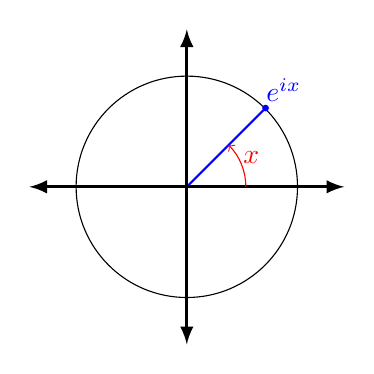
\begin{tikzpicture}
        \draw[blue, thick] (0, 0) -- (1, 1);
        \draw[latex-latex, very thick] (-2, 0) -- (2, 0);
        \draw[latex-latex, very thick] (0, -2) -- (0, 2);
        \draw[smooth] (0, 0) circle (40pt);
        \draw[fill = blue, draw = blue] (1, 1) circle (1pt);
        \draw[->,red] (0.75, 0) arc(0:45:0.75);
        \node[text = red] at (0.82, 0.37) {$x$};
        \node[text = blue] at (1.23, 1.23) {$e^{ix}$};

    \end{tikzpicture}
    
    \caption{Visualization of the map $x \mapsto e^{ix}$ from $[0, 2\pi)$ onto the unit circle in the complex plane.}
    \label{fig55}
\end{figure}


\subsection{The Algebraic Completeness of the Complex Field}

\setcounter{rudin}{7}

\begin{theorem}{The Fundamental Theorem of Algebra}{}
    Let $n \in \NN$, and $a_0, a_1, \ldots, a_n \in \CC$ such that $a_n \neq 0$. Define the polynomial:
    \begin{align*}
        P(z) = a_0 + a_1z + \ldots + a_nz^n
    \end{align*}
    with $z \in \CC$. Then, there exists $z_0 \in \CC$ such that $P(z_0) = 0$. 
\end{theorem}

\begin{ncorollary}{}{}
    By division, $P_n(z)$ has $n$ roots. 
\end{ncorollary}

\begin{nproof}
    Assume WLOG that $a_n = 1$ (this can be realized by dividing out by the original nonzero $a_n$). Let $\mu = \inf_{z \in \CC}\abs{P(z)}$. We wish to show that $\mu = 0$, and that the inf is attained at some $z_0 \in \CC$. 

    We first show that the infimum is attained. The idea of the argument is that for large $z$, $z^n$ grows the most rapidly and hence it dominates. Hence, $\abs{P(z)}$ is large. Hence, the $\inf$ is attained in some compact disk, but since $P$ is continuous, the $\inf$ is therefore obtained somewhere on this compact set. Formally, for $\abs{z} = R$, we have that:
    \begin{align*}
        \abs{P(z)} = \abs{z^n}\abs{\frac{a_0}{z^n} + \frac{a_1}{z^{n-1}} + \ldots + \frac{a_{n-1}}{z} + 1} &\geq \abs{z}^n\left(1 - \frac{\abs{a_0}}{\abs{z}^n} - \frac{\abs{a_1}}{\abs{z}^{n-1}} - \ldots - \frac{\abs{a_{n-1}}}{\abs{z}}\right)
        \\ &= R^n\left(1 - \frac{\abs{a_0}}{\abs{z}^n} - \frac{\abs{a_1}}{\abs{z}^{n-1}} - \ldots - \frac{\abs{a_{n-1}}}{\abs{z}}\right)
    \end{align*}
    We see that this expression goes to infinity as $R \rightarrow \infty$. Hence, $\abs{P(z)} \geq \mu + 1$ if $\abs{z} \geq R_0$ for some $R_0 > 0$. As $\abs{P}$ is continuous, and $\abs{z} \leq R_0$ is a compact subset of $\CC$, $\mu$ is attained somewhere on the subset by the Extreme Value Theorem (Theorem \ref{thm:4.16}). Therefore, $\mu = \abs{P(z_0)}$ for some $z_0$ with $\abs{z_0} \leq R_0$. 

    Next, we show that $\mu = 0$. Suppose (for the sake of contradiction) that $\mu > 0$ and hence $P(z_0) \neq 0$. Let $Q(z) = \frac{P(z_0 + z)}{P(z_0)}$. Then $Q(0) = 1$, so:
    \begin{align*}
        Q(z) = 1 + b_kz^k + \ldots + b_nz^n
    \end{align*}
    where $b_k$ is the first nonzero coeffient. Furthermore, we see that $\abs{Q(z)} = \frac{\abs{P(z_0 + z)}}{\mu} \geq 1$ for all $z \in \CC$ (as $\mu$ is the infimum). We will now derive a contradiction by looking at small $z$ (where $z^k > z^{k+1} > \ldots > z^n$). We consider that:
    \begin{align*}
        \abs{Q(z)} \leq \abs{1 + b_kz^k} + \sum_{m=k+1}^n \abs{b_m}\abs{z^m}
    \end{align*}
    We want to choose $z$ small enough such that the first term in the above expression is less than $1$ and the others are negligeble. To this end, let us write $bk = \frac{b_k}{\abs{b_k}}\abs{b_k} = e^{it_1}\abs{b_k}$ for some $t_1 \in \RR$. Then, let $t = \frac{-t_1 + \pi}{k}$ so $t_1 = -kt + \pi$. We then have that $b_k = -e^{-itk}\abs{b_k}$ (where the minus sign comes from $e^{i\pi}$). Choose $z = re^{it}$ with $r > 0$. Then, $z^k = r^ke^{itk}$ and $b_kz^k = -e^{-itk}\abs{b_k}r^ke^{itk} = -r^k\abs{b_k} < 0$. Let us choose $r$ small enough so that $\abs{b_k}r^k < 1$ is satisfied. We then have that:
    \begin{align*}
        \abs{1 + b_kz^k} = \abs{1 - \abs{b_k}r^k} = 1 - \abs{b_k}r^k
    \end{align*}
    so therefore:
    \begin{align*}
        \abs{Q(z)} \leq 1 - \abs{b_k}r^k + \sum_{m=k+1}^n \abs{b_m}r^k = 1 - r^k\left(\abs{b_k} - r\abs{b_{k+1}} - \ldots - r^{n-k}\abs{b_n}\right)
    \end{align*}
    where $\left(\abs{b_k} - r\abs{b_{k+1}} - \ldots - r^{n-k}\abs{b_n}\right) > 0$. Hence $\abs{Q(z)} < 1$, which is a contradiction. We conclude that $\abs{P(z_0)} = 0$. \qed
\end{nproof}

\subsection{Fourier Series}
\noindent We now begin our discussion on Fourier Series. Note that the theory of Fourier Series (and more generally, Harmonic Analysis) is rich enough for it to be its own course, but we will here give an introduction to the topic. Fourier Series show up everywhere, such as (for example) in partial differential equations, or in signal processing. It is an interesting topic of study that combines analysis and linear algebra. 

For some additional references on the topic, Katznelson's ``Harmonic Analysis'' (\url{https://www.cambridge.org/core/books/an-introduction-to-harmonic-analysis/67C4CE356E7420BA17F3F1337291EF82}) and 

\noindent Grafakos' ``Classical Fourier Analysis'' (\url{https://link.springer.com/book/10.1007/978-1-4939-1194-3}) are good texts.

\begin{ndef}{: Inner Product/Norm of Functions}{}
    Given $a, b \in \RR$ with $a < b$ and integrable $f, g: [a, b] \mapsto \CC$ we write:
    \begin{align*}
        \avg{f, g} = \int_a^b f(x)\overline{g(x)}dx \; \left(= \overline{\avg{g, f}}\right)
    \end{align*}
    to denote the inner product on the space of complex functions. Note that this inner product induces the norm $\norm{f}_2 = \sqrt{\avg{f, f}} = \left(\int_a^b \abs{f(x)}^2 dx\right)^{1/2}$. 

    Note that we will often take $[a, b] = [0, 2\pi]$ and in this case we may prefer:
    \begin{align*}
        \avg{f, g} = \frac{1}{2\pi}\int_0^{2\pi}f(x)\overline{g(x)}dx.
    \end{align*} 
\end{ndef}
\noindent As a remark, we have that $d(f, g) = \norm{f - g}_2$ induces a metric, but we have to be careful; it defines a metric on the metric space of continuous functions (that is, $\C[a, b]$) but \emph{not} as on the space of Riemann-integrable functions (i.e. $\R[a, b]$). To see this, consider that we can have $f \in \R[a, b]$ with $\int_a^b \abs{f(x)}dx = 0$ but $f \neq 0$ (consider any function $f$ which is zero everywhere but is nonzero for a finite number of points). 

\begin{ndef}{: Orthogonal/Orthonormal Families of Functions}{}
    We say that a family of functions $\phi_n [a, b] \mapsto \CC$ are mutually \textbf{orthogonal} if:
    \begin{align*}
        \avg{\phi_n, \phi_m} = 0 \text{ if $n \neq m$.}
    \end{align*}
    We say that a family of functions is \textbf{orthonormal} if:
    \begin{align*}
        \avg{\phi_n, \phi_m} = \delta_{nm} = \begin{cases}
            1 & n = m
            \\ 0 & n \neq m
        \end{cases}.
    \end{align*}
\end{ndef}

\begin{nexample}{}{}
    \begin{enumerate}
        \item Let $[a, b] = [-\pi, \pi]$. Then, $\phi_n(x) = \frac{1}{\sqrt{2\pi}}e^{inx}$, $n \in \ZZ$ obey:
        \begin{align*}
            \avg{\phi_n, \phi_m} = \frac{1}{2\pi}\int_{-\pi}^\pi e^{i(m-n)x}dx = \frac{1}{2\pi}\int_{-\pi}^\pi\cos((m-n)x) + i\sin((m-n)x)dx = \delta_{nm}.
        \end{align*}
        \item Take $\phi_1, \phi_2, \ldots$ to be $\frac{1}{\sqrt{2\pi}}, \frac{1}{\sqrt{2\pi}}\cos(x),  \frac{1}{\sqrt{2\pi}}\sin(x),  \frac{1}{\sqrt{2\pi}}\cos(2x), \ldots$. We then have that this family is orthonormal on $[-\pi, \pi]$. 
        \item The Legendre polynomials, defined by $P_n(x) = \sum_{k=0}^n \binom{n}{k}\binom{n+k}{n}\left(\frac{x - 1}{2}\right)^k$ for $n \in \NN \cup \set{0}$ are orthogonal on $[-1, 1]$. Note that $\norm{P_n}_2 = \sqrt{\frac{2}{2n+1}}$. 
    \end{enumerate}
\end{nexample}
\noindent With this definition defined, we will want to use sets of orthonormal functions as a \emph{basis} of $L^2$ space. We want to be able to write arbitrary $f \in L^2$ as a linear combination of these functions.

\begin{nexample}{}{}
    As motivation for the next definition, suppose $f(x) = \sum_{m=0}^N c_n \phi_n$ with $\set{\phi_n}$ orthonormal on $[a, b]$. Then, we can write:
\begin{align*}
    \avg{f, \phi_n} = \sum_{m=0}^N c_m \avg{\phi_m, \phi_n} = \sum_{m=0}^NN c_m \delta_{mn} = c_n.
\end{align*}
That is, we can write $c_n = \avg{f, \phi_n} = \int_a^b f(x)\overline{\phi_n(x)}dx$.

As a specific example, suppose $f(x) = \sum_{n=-N}^N c_ne^{inx} = \sum_{n=-N}c_n\sqrt{2\pi}\frac{e^{inx}}{\sqrt{2\pi}}$. From the previous example, we have that $\frac{e^{inx}}{\sqrt{2\pi}}$ is orthonormal on $[-\pi, \pi]$. Hence:
\begin{align*}
    \sqrt{2\pi}c_n = \avg{f, \phi_n} = \frac{1}{\sqrt{2\pi}}\int_{-\pi}^\pi f(x)e^{inx}.
\end{align*}
That is, $c_n = \frac{1}{2\pi}\int_{-\pi}^\pi f(x)e^{-inx}dx$. 
\end{nexample}

\begin{ndef}{: Fourier Coefficients/Series}{}
    If $f \in \R[a, b]$ and $\set{\phi_n}$ is an orthonormal family of functions, then $c_n = \avg{f, \phi_n}$ is called a \textbf{Fourier coefficient of $f$}, and the \textbf{Fourier series of $f$} is $\sum_n c_n \phi_n$. 
\end{ndef}
\noindent A natural question after making this definition is ``when does the Fourier series of $f$ converge?'' A follow-up question is ``when it converges, is it equal to $f$?'' We will investigate these questions with the next sequence of theorems.

\setcounter{rudin}{10}

\begin{theorem}{}{8.11}
    Suppose $f \in \R[a, b]$ and $\set{\phi_n}$ is an orthonormal on $[a, b]$. Let $c_n = \avg{f, \phi_n}$ and $s_n = \sum_{m=1}^n c_m\phi_m$. Let $t_n = \sum_{m=1}^n a_m\phi_m$ for some $a_m \in \CC$. Then, we have that:
    \begin{align*}
        \norm{f- s_n}_2^2 \leq \norm{f - t_n}_2^2
    \end{align*}
    with equality if and only if $c_m = a_m$ for each $m$. 
\end{theorem}
\noindent The moral of the theorem is that if we are to use a linear combination of the first $n$ functions out of an orthonormal set of functions to best approximate $f$ in the $L^2$ norm, the best way to do so is by using Fourier coefficients. 

\begin{nproof}
    By the definition of the norm, we have that:
    \begin{align*}
        \norm{f - t}_2^2 = \avg{f - t_n, f - t_n}^2 = norm{f}_2^2 - \avg{t_n, f} - \avg{f, t_n} + \norm{t_n}_2^2
    \end{align*}
    Looking at the terms, we have that:
    \begin{align*}
        \norm{t_n}_2^2 = \avg{t_n, t_n} = \sum_{k, m = 1}^n a_k\overline{a_m}\avg{\phi_k, \phi_m} = \sum_{k, m = 1}^n a_k\overline{a_m}\delta_{km} = \sum_{m=1}^n a_m\overline{a_m} \quad (1)
    \end{align*}
    \begin{align*}
        \avg{f, t_n} = \sum_{m=1}^n \overline{a_m}\avg{f, \phi_n} = \sum_{m=1}^n c_m\overline{a_m}
    \end{align*}
    Therefore:
    \begin{align*}
        \norm{f - t_n}_2^2 &= \norm{f}_2^2 + \sum_{m=1}^n a_m\overline{a_m} - c_m\overline{a_m} - \overline{c_m}a_m 
        \\ &= \norm{f}_2^2 + \sum_{m=1}^n \left(a_m\overline{a_m} - c_m\overline{a_m} - \overline{c_m}a_m + c_m\overline{c_m}\right) - \sum_{m=1}^n c_m\overline{c_m}
        \\ &= \norm{f}_2^2 + \sum_{m=1}^n \abs{a_m - c_m}^2 - \sum_{m=1}^n \abs{c_m}^2
    \end{align*}
    Putting $a_m = c_m$, we obtain:
    \begin{align*}
        \norm{f - s_n}_2^2 = \norm{f}_2^2 - \sum_{m=1}^n \abs{c_m}^2. \quad (2)
    \end{align*} Hence, we have that:
    \begin{align*}
        \norm{f - t_n}_2^2 = \norm{f - s_n}_2^2 + \sum_{m=1}^n \abs{a_m - c_m}^2
    \end{align*} 
    And $\sum_{m=1}^n \abs{a_m - c_m}^2 \geq 0$ and is $0$ if and only if $a_m = c_m$ for all $m$. This proves the claim. \qed
\end{nproof}
\noindent Note that putting $(1)$ and $(2)$ together in the above proof give the identity that $\norm{f}_2^2 = \norm{f - s_n}_2^2 + \norm{s_n}_2^2$. There is a geometric interpretation to this identity, which we picture below:

\begin{figure}[htbp]
    \centering
    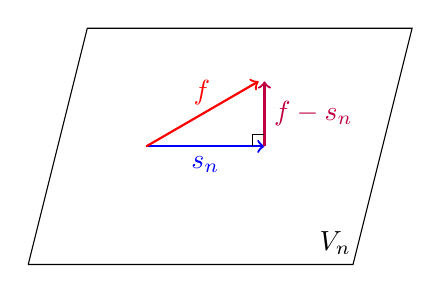
\begin{tikzpicture}[scale=1.5]
        \draw[] (0, 0) -- (2.75, 0) -- (3.25, 2) -- (0.5, 2) -- (0, 0);
        \draw[->, thick, blue] (1, 1) -- (2, 1);
        \draw[->, thick, purple] (2, 1) -- (2, 1.55);
        \draw[->, thick, red] (1, 1) -- (1.95, 1.55);
        \draw[] (1.9, 1) -- (1.9, 1.1) -- (2, 1.1);
        \node[text = red, above] at (1.47, 1.27) {$f$};
        \node[text = blue, below] at (1.5, 1) {$s_n$};
        \node[text = purple, right] at (2, 1.28) {$f - s_n$};
        \node[above] at (2.6, 0) {$V_n$};
    \end{tikzpicture}
    
    \caption{Visualization of the identity $\norm{f}_2^2 = \norm{f - s_n}_2^2 + \norm{s_n}_2^2$. If we let $V_n$ be the set of all linear combinations of $\phi_1, \ldots, \phi_n$ (i.e. all sums of the form $\sum_{m=1}^n a_m\phi_m$), then $s_n$ is the orthogonal projection of $f$ onto $V_n$.}
    \label{fig55}
\end{figure}

\begin{theorem}{Bessel's Inequality}{8.12}
    Suppose $\set{\phi_n}$ is orthonormal on $[a, b]$ and is an infinite family. If $f(x) = \sum_{n=1}^\infty c_n \phi_n$, then:
    \begin{align*}
        \sum_{n=1}^\infty \abs{c_n}^2 \leq \int_a^b \abs{f(x)}^2 dx.
    \end{align*}
    We call this the Bessel Inequality. Note that this implies:
    \begin{align*}
        \linf c_n = 0
    \end{align*}
\end{theorem}

\begin{nproof}
    We start with the identity that $\norm{f}_2^2 = \norm{f - s_n}_2^2 + \norm{s_n}_2^2$. It then follows that $\sum_{m=1}^n \abs{c_m}^2 = \norm{s_m}_2^2 \leq \norm{f}_2^2$. We then take $n \rightarrow \infty$. Since $\sum_{m=1}^n \abs{c_m}$ is bounded above (by $\norm{f}_2^2$) for any $n$ and is monotonically increasing, we conclude that the infinite series converges and hence:
    \begin{align*}
        \sum_{n=1}^\infty \abs{c_n}^2 \leq \int_a^b \abs{f(x)}^2 dx.
    \end{align*}
    By the divegence test (Theorem \ref{thm:3.23}) we obtain that $\linf c_n = 0$. \qed
\end{nproof}

\begin{nexample}{}{}
    Suppose $f \in \R[-\pi, \pi]$. Then, $\linf \int_{-\pi}^{\pi} f(x)\cos(nx) dx = 0$ by the above Theorem. 
\end{nexample}
\noindent The above example is a version of the Riemann-Lebesgue Lemma. The intuitive interpretation of the above example is that $\cos(nx)$ oscillates wildly as $n \rightarrow \infty$, and hence under the integral, the peaks/valleys cancel.

\begin{ndef}{: Inner Product/Norm of Functions (Revisited)}{}
    From now on, we will restrict ourselves to $f: [-\pi, \pi] \mapsto \CC$ with $f \in \R[-\pi, \pi]$. Take $\phi_n(x) = e^{inx}$ for $n \in \ZZ$. We extend $f$ to all of $\RR$ by $f(x + 2\pi) = f(x)$. To make the $\phi_n$s orthonormal over our interval, we change our definition of our inner product and norm:
    \begin{align*}
        \avg{f, g} = \frac{1}{2\pi}\int_{-\pi}^\pi f(x)\overline{g(x)}dx, \norm{f}_2^2 = \avg{f, f} = \frac{1}{2\pi}\int_{-\pi}^\pi\abs{f(x)}^2 dx
    \end{align*}
    We then have that $\avg{\phi_n, \phi_m} = \delta_{nm}$. Theorem \ref{thm:8.11} and its consequences hold with this new definition.
\end{ndef}

\begin{ndef}{: Fourier Series (Revisited)}{}
    We define the \textbf{Fourier series} of $f$ by:
    \begin{align*}
        \sum_{n=-\infty}^\infty c_n\phi_n(x)
    \end{align*}
    where $c_n = \avg{f, \phi_n}$ and $\phi_n(x) = e^{inx}$.
\end{ndef}
\noindent Note that at this point, we do note claim that the Fourier series converges, nor that it equals $f$.

\begin{ndef}{: Partial Fourier Series}{}
    The $N$th partial Fourier seris of $f$ is defined as $s_N(f;x) = \sum_{n=-N}^N c_ne^{inx}$. Where $f$ is clear from context, we sometimes will write $s_N(x)$.
\end{ndef}
\noindent Note that Theorem \ref{thm:8.12} implies that:
\begin{align*}
    \sum_{n = -N}^{N} \abs{c_n}^2 = \norm{s_N}_2^2 \leq \norm{f}_2^2.
\end{align*}

\begin{ndef}{: The Dirchlet Kernel}{}
    The \textbf{Dirchlet Kernel} is defined as:
    \begin{align*}
        D_n(t) = \sum_{n=-N}^{N}e^{int}.
    \end{align*}
\end{ndef}

\begin{nlemma}{ 1}{}
    $D_n(t) = \frac{\sin((N + \frac{1}{2})t)}{\sin(\frac{1}{2}t)}$.
\end{nlemma}

\begin{nproof}
    By definition, we have that $D_N(t) = \sum_{n=-N}^N e^{int}$. We then have that:
    \begin{align*}
        D_N(t) &= \sum_{n=-N}^N e^{int}
        \\ &= e^{-iNt}\sum_{k=0}^{2N}(e^{it})^k & \text{(Common factor)}
        \\ &= e^{-iNt}\left[\frac{e^{i(2N+1)} - 1}{e^{it} - 1}\right] & \text{(Geometric sum)}
        \\ &= e^{-iNt}\left[\frac{e^{i(2N+1)} - 1}{e^{it} - 1}\right]\frac{e^{-it/2}}{e^{-it/2}}
        \\ &= \frac{e^{i(N+1/2)t} - e^{-i(N+1/2)t}}{e^{it/2} - e^{-it/2}}
        \\ &= \frac{\sin((N + \frac{1}{2})t)}{\sin(\frac{1}{2}t)}
    \end{align*} \qed
\end{nproof}

\begin{figure}[htbp]
    \centering
    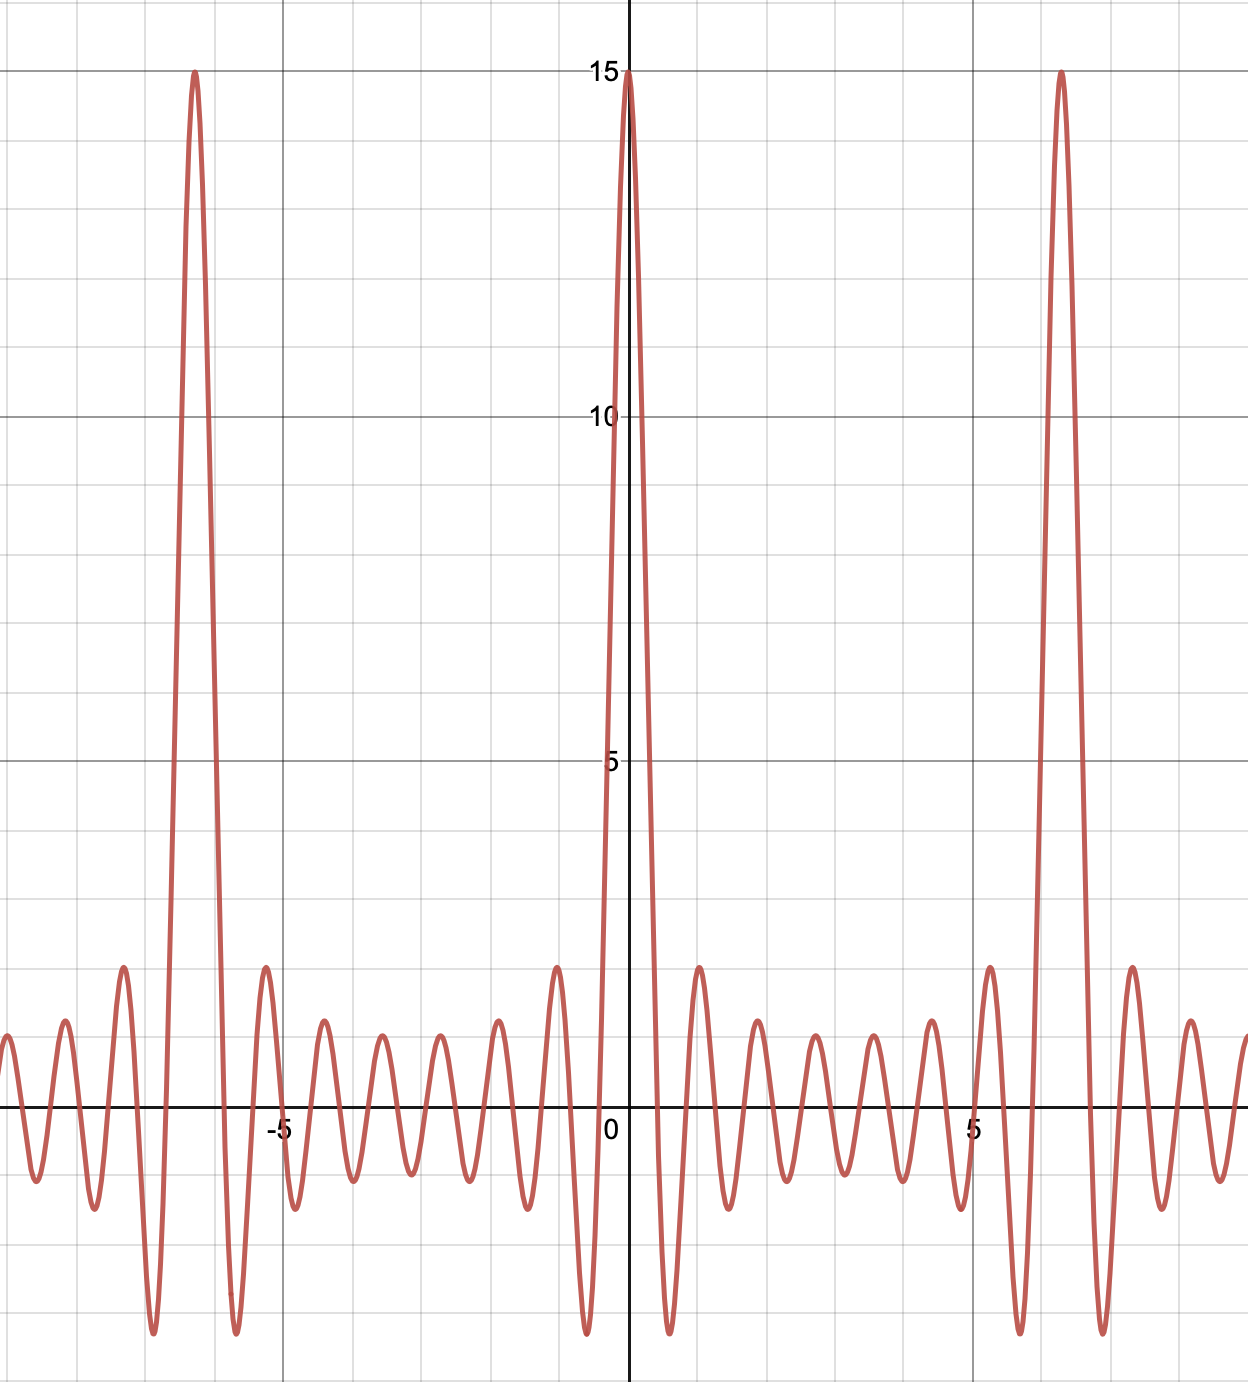
\includegraphics[scale=0.3]{Images/Dirchlet-graph.png}
    
    \caption{Desmos Visualization of the Dirchlet Kernel $D_N(t)$ for $N = 7$. $D_N(t)$ is $2\pi$ periodic, and becomes more sharply peaked at $t = \pi n$, $n \in \ZZ$ as we increase $N$. It can be understood as an oscillating function that approaches a $\delta$ ``function''. Readers can play around with the function at \url{https://www.desmos.com/calculator/satukmy8kj}.}
    \label{fig56}
\end{figure}

\begin{nlemma}{ 2}{}
    For $x \in \RR$, $s_N(f;x) = \frac{1}{2\pi}\int_{-\pi}^\pi f(x - t)D_N(t)dt$.
\end{nlemma}
\noindent What we would like to see is that $s_N(f;x) \rightarrow f$ as $N \rightarrow \infty$. Given the above Lemma, this can be realized if $D_N(t) \rightarrow \delta(t)$ (where $\delta(t)$ is the Dirac delta ``function''; of course this is not actually a function, but the intuition is that $D_N(t)$ becomes sharply peaked around $t$) and then $f(x - t) = f(x)$. Note that the integral formula above is of a \emph{convolution integral}. We will discuss properties of it and the Dirchlet kernel, and use it to show that $s_N \rightarrow f$ if $f$ is Lipschitz continuous.

\begin{nproof}
    By calculation and algebraic manipulation, we have that:
    \begin{align*}
        s_N(x) = \sum_{n=-N}^N c_ne^{inx} &= \sum_{n=-N}^{N}\avg{f, \phi_n}e^{inx}
        \\ &= \sum_{n=-N}^N \frac{1}{2\pi}\int_{-\pi}^\pi f(t)e^{-int}dt e^{inx}
        \\ &= \sum_{n=-N}^N \frac{1}{2\pi}\int_{-\pi}^\pi f(t)e^{in(x - t)} dt
        \\ &= \frac{1}{2\pi}\int_{-\pi}^\pi f(t)\sum_{n=-N}^N e^{in(x-t)} dt 
        \\ &= \frac{1}{2\pi} \int_{-\pi}^\pi f(t)D_N(x - t)dt 
        \\ &= \frac{1}{2\pi}\int_{x - \pi}^{x + \pi}f(x - s)D_N(s)ds & \text{(Substitute $s = x - t$)}
        \\ &= \frac{1}{2\pi}\int_{- \pi}^{\pi}f(x - s)D_N(s)ds & \text{(Periodicity of $f, D_N$)}
    \end{align*} \qed
\end{nproof}

\begin{nlemma}{ 3}{}
    \begin{enumerate}
        \item $\frac{1}{2\pi}\int_{-N}^N D_N(t)dt = 1$
        \item $D_N(t) = \cos(nt) + \cot(\frac{1}{2}t)\sin(nt)$. 
    \end{enumerate}
\end{nlemma}
\begin{nproof}
    \begin{enumerate}
        \item $\frac{1}{2\pi}\int_{-N}^N D_N(t)dt = \avg{D_N, 1} = \sum_{n=-N}^N \avg{\phi_n, \phi_0} = \sum_{n=-N}^N \delta_{N_0} = 1$.
        \item $D_N(t) = \frac{1}{\sin(\frac{1}{2}t)}\left(\sin(\frac{1}{2}t)\cos(Nt) + \cos(\frac{1}{2}t)\sin(Nt)\right) = \cos(nt) + \cot(\frac{1}{2}t)\sin(nt)$. \qed
    \end{enumerate}
\end{nproof}

\setcounter{rudin}{13}
\begin{theorem}{}{8.14}
    Let $x \in \RR$, $f \in \RR$ on $[-\pi, \pi]$. Suppose there exist $\delta > 0$, $M < \infty$ such that $\abs{f(x + t) - f(x)} \leq M\abs{t}$ for all $\abs{t} < \delta$. Then, we have that $\lim_{N \rightarrow \infty} s_N(x) = f(x)$.
\end{theorem}

\begin{figure}[htbp]
    \centering
    \begin{tikzpicture}[scale=1.5]
        \draw[-latex, very thick] (0, 0) -- (2, 0);
        \draw[-latex, very thick] (0, 0) -- (0, 2);
        \draw[] (1, 0) -- (1, -0.15);
        \node[below] at (1, -0.17) {$x$};
        \draw[] (0.5, 0) -- (0.5, -0.15);
        \node[below] at (0.5, -0.12) {$x - \delta$};
        \draw[] (1.5, 0) -- (1.5, -0.15);
        \node[below] at (1.5, -0.12) {$x + \delta$};
        \draw[dotted] (0.5, 0.75) -- (1.5, 1.25);
        \draw[dotted] (0.5, 1.25) -- (1.5, 0.75);
        \draw[blue] (0.25, 0.6) to [curve through ={(0.5, 0.9)..(0.75, 1.1)..(0.9,1)..(1, 1)..(1.1,1)..(1.25, 0.9)...(1.5, 1.1)}] (1.6, 1.6);
        \node[text = blue, right] at (1.5, 1) {$f$};
    \end{tikzpicture}
    
    \caption{Visualization of the Lipschitz continuity condition on $f$ in Theorem \ref{thm:8.14}. $f$ is bounded in between lines of slope $\pm M$ for a neighbourhood $N_\delta(x)$ around $x$.}
    \label{fig57}
\end{figure}

\begin{nproof}
    We show that $f(x) - s_N(x)$ goes to zero. The intuition for the proof we will use is that $D_N(t)$ will behave like a delta function, picking out a specific value of $x$. Using the result of the previous Lemma, we have:
    \begin{align*}
        f(x) - s_N(x) &= f(x)\frac{1}{2\pi}\int_{-\pi}^\pi D_N(t)dt - \frac{1}{2\pi}\int_{-\pi}^\pi f(x-t)D_N(t)dt & \text{Lemma 3(a)/2}
        \\ &= \frac{1}{2\pi}\int_{-\pi}^\pi (f(x) - f(x - t))D_N(t) dt & \text{Theorem \ref{thm:6.12}}
        \\ &= \frac{1}{2\pi}\int_{-\pi}^\pi (f(x) - f(x - t))\cos(Nt)dt & \text{Lemma 2(a)}
        \\ &+ \frac{1}{2\pi}\int_{-\pi}^\pi (f(x) - f(x-t))\cot(\frac{1}{2}t)\sin(Nt)dt 
    \end{align*}
    The first term is easy; by the Riemann-Lebesgue Lemma (see the example after Theorem \ref{thm:8.12}), since $f(x) - f(x - t)$ is Riemann integrable, we have that the first term goes to $0$ as $N \rightarrow \infty$. For the second term, we show that $(f(x) - f(x-t))\cot(\frac{1}{2}t)$ is Riemann-integrable and then use the Riemann-Lebesegue Lemma again. We have that:
    \begin{align*}
        (f(x) - f(x-t))\cot(\frac{1}{2}t) = \frac{f(x) - f(x-t)}{t} \frac{\frac{t}{2}}{\sin(\frac{t}{2})}2\cos(\frac{t}{2})
    \end{align*}
    where $\frac{f(x) - f(x-t)}{t}$ is bounded by $M$ by the Lipschitz continuity assumption at $x$, $\frac{\frac{t}{2}}{\sin(\frac{t}{2})} \rightarrow 1$ as $t \rightarrow 0$ and is bounded and continuous, and $2\cos(\frac{t}{2})$ is of course continuous. Hence, $(f(x) - f(x-t))\cot(\frac{1}{2}t)$ is Riemann Integrable, and we conclude that the second term also goes to $0$ as $N \rightarrow \infty$. Hence $\lim_{N \rightarrow \infty}f(x) - s_N(x) = 0$. \qed
\end{nproof}

\begin{ntheorem}{}{}
    The partial sum $s_N$ is linear in $f$.
\end{ntheorem}
\begin{nproof}
    Recall the definition that $s_N(f;x) = \sum_{n=-N}^N \avg{f, \phi_n}\phi_n(x)$. Using the linearity of the inner product in the first argument, we then have that:
    \begin{align*}
        s_N(af + bg; x) &= \sum_{n=-N}^N \avg{af + bg, \phi_n}\phi_n(x)
        \\ &= a\sum_{n=-N}^N \avg{f, \phi_n} + b\sum_{n = -N}^N \avg{g, \phi_n}\phi_n(x)
        \\ &= as_N(f;x) + bs_N(g;x)
    \end{align*}
    so $s_N$ is linear in $f$ as claimed. \qed
\end{nproof}
\noindent With linearity established, we give a corollary of Theorem \ref{thm:8.14}.

\begin{ncorollary}{}{}
    \begin{enumerate}
        \item If $f(x) = 0$ for all $x \in (x_0 - \e, x_0 + \e)$ then $s_N(f;x) \rightarrow 0$ for all such $x$ (the Theorem can be immediately applied as $\abs{f(x + t) - f(x)} < M\abs{t}$ is satisfied for all constant $x$).
        \item If $f(x) = g(x)$ for all $x \in (x_0 - \e, x_0 + \e)$ then by the linearity of $s_N$ in $f$ we have that $s_N(f;x) - s_N(g;x) \rightarrow 0$ for all such $x$.
    \end{enumerate}
\end{ncorollary}

\begin{figure}[htbp]
    \centering
    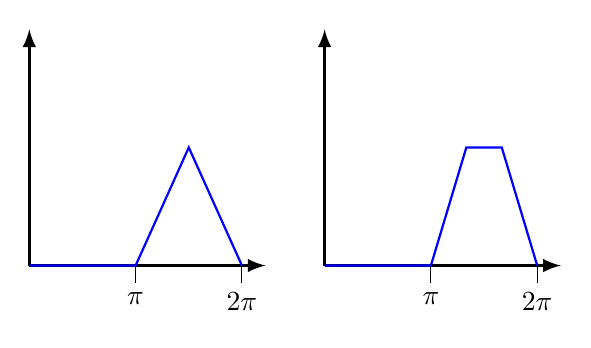
\begin{tikzpicture}[scale=1.5]
        \draw[-latex, very thick] (0, 0) -- (2, 0);
        \draw[-latex, very thick] (0, 0) -- (0, 2);
        \draw[-latex, very thick] (2.5, 0) -- (4.5, 0);
        \draw[-latex, very thick] (2.5, 0) -- (2.5, 2);
        \draw[] (0.9, 0) -- (0.9, -0.15);
        \node[below] at (0.9, -0.15) {$\pi$};
        \draw[] (1.8, 0) -- (1.8, -0.15);
        \node[below] at (1.8, -0.15) {$2\pi$};
        \draw[] (3.4, 0) -- (3.4, -0.15);
        \node[below] at (3.4, -0.15) {$\pi$};
        \draw[] (4.3, 0) -- (4.3, -0.15);
        \node[below] at (4.3, -0.15) {$2\pi$};
        \draw[blue, thick] (0, 0) -- (0.9, 0) -- (1.35, 1) -- (1.8, 0);
        \draw[blue, thick] (2.5, 0) -- (3.4, 0) -- (3.7, 1) -- (4, 1) -- (4.3, 0);
    \end{tikzpicture}
    
    \caption{Two functions to which we can apply the above corollary. The two functions have different Fourier series, but both series converge to zero on $[0, \pi]$. This is very different behaviour from power series, see for example Theorem \ref{thm:8.5}. This corollary/example shows off the ``localization principle'' of Fourier series.}
    \label{fig58}
\end{figure}

\begin{theorem}{}{8.15}
    If $f$ is continuous and has period $2\pi$, then for all $\e > 0$ there exists a trigonometric polynomial $P(x) = \sum_{n=-N}^N a_ne^{inx}$ such that $\sup_{x \in \RR}\abs{f(x) - P(x)} < \e$.
\end{theorem}
\noindent Note that the above theorem does \emph{not} imply that Fourier series converge uniformly.

\begin{nproof}
    Let $T = \set{z \in \CC: \abs{z} = 1}$ (i.e. the unit circle in the complex plane). $T$ is compact. Define $F: T \mapsto \CC$ by $F(e^{ix}) = F(x)$. By the periodicity of $f$, $F$ is well defined. Let $\A$ be the set of trig polynomials $\sum_{n=-N}^N a_nz^n$ with $z \in T$ and $a_n \in \CC$. We show that $\A$ satisfies the conditions for the (complex) Stone-Weierstrass theorem to be applied. $\A$ is closed under addition and multiplication (as is easily verified by condidering the sum/products of finite sums). $\A$ vanishes at no point in $T$ as $1 \in \A$. $\A$ separates points in $T$ as $f(x) = x \in \A$. $\A$ is self-adjoint as if $\sum_{n=-N}^N a_nz_n \in \A$:
    \begin{align*}
        \overline{\sum_{n=-N}^N a_nz_n,} = \sum_{n=-N}^N \overline{a_n}\overline{z}^n = \sum_{n=-N}^N \overline{a_n}z^{-n} = \sum_{m=-N}^N \overline{a_m}z^{m} \in \A
    \end{align*}
    where we let $m = -n$. Hence, by the Stone-Weierstrass theorem (Theorem \ref{thm:7.33}) there exists $P \in \A$ such that $\abs{F(z) - P(z)} < \e$ for all $z \in T$. Write $P(z) = \sum_{n=-N}^N a_nz^n$ and set $P(x) = P(e^{ix}) = \sum_{n=-N}^N a_ne^{inx}$. Then, we have that $\abs{f(x) - p(x)} = \abs{F(e^{ix}) - P(e^{ix})} < \e$. for all $x \in \RR$. \qed
\end{nproof}

\noindent Note that problem 8.15 gives an explicit sequence of trigonometric polynomials that converge uniformly to $f$. 

As a point of notation for the next theorem, for $\set{c_n}_{n \in \ZZ}$ and $\set{\gamma_n}_{n \in \ZZ}$, let $(c, \gamma) = \sum_{n=-N}^N c_n\overline{\gamma_n}$. Note that there is no guarantee that this sum converges. Furthermore, let us review the notation that we have already established. $\avg{f, g} = \frac{1}{2\pi}\int_{-\pi}^\pi f(x)\overline{g(x)}dx$, $\norm{f}_2 = \sqrt{\avg{f, f}}$ (when the integral converges), $\phi_n(x) = e^{inx}$. $s_N(f;x) = \sum_{n=-N}^N \avg{f, \phi_n}\phi_n$. 

\begin{ntheorem}{: Cauchy Shwartz Inequality for Norms (Problem 6.10)}{}
    $\abs{\avg{f, g}} \leq \norm{f}_2\norm{g}_2$.
\end{ntheorem}

\begin{ntheorem}{: Minkowski Inequality (Problem 6.11)}{}
    $\norm{f + g}_2 \leq \norm{f}_2 + \norm{g}_2$, and $\norm{f - g}_2 \leq \norm{f - h}_2 + \norm{h - g}_2$.
\end{ntheorem}

\begin{ntheorem}{ (Problem 6.12)}{}
    For $f \in \R[-\pi, \pi]$ and $\e > 0$, there exists a continuous (in fact, piecewise linear) function $h$ such that $\norm{f - h}_2 < \e$.
\end{ntheorem}

\begin{nproof}
    Left as an exercise. Solutions to the problems can be found at \url{https://minds.wisconsin.edu/bitstream/handle/1793/67009/rudin%20ch%206.pdf?sequence=6&isAllowed=y}. \qed
\end{nproof}

\begin{theorem}{Parseval's Relation \& The Bessel Equality}{8.16}
    For $f, g \in \R[-\pi, \pi]$, let $c_n = \avg{f, \phi_n}$ and $\gamma_n = \avg{g, \phi_n}$. Then $\lim_{N \rightarrow \infty}\norm{f - s_N(t)} = 0$ (Convergence of partial Fourier series to $F$ in $L_2$). Furthermore, $\avg{f, g} = (c, \gamma)$ (Parseval's Relation) and in particular $\norm{f}_2^2 = (c, c)$. I.e. $\frac{1}{2\pi}\int_{-\pi}^\pi \abs{f(x)}^2dx = \sum_{n=-\infty}^\infty \abs{c_n}^2$ (Bessel Equality).
\end{theorem}

\begin{nproof}
    Let $\e > 0$. Choose a continuous $h$ such that $\norm{f- h}_2 < \frac{\e}{3}$ (Problem 6.12). Then:
    \begin{align*}
        \norm{s_N(f;x) - f}_2 \leq \norm{s_N(f;x) - s_N(h;x)}_2 + \norm{s_N(h;x) - h}_2 + \norm{h - f}_2.
    \end{align*}
    We have that the third term is less than $\frac{\e}{3}$ by assumption. For the first term, by the linearity of $s_N$ we have that $\norm{s_N(f;x) - s_N(h;x)} = \norm{s_N(f - h)}_2 \leq \norm{f-h}_2 < \frac{\e}{3}$ (using Bessel's Inequality). For the second term, by Theorem \ref{thm:8.15} we have that there exists a trigonometric polynomial $P$ such that $\norm{h - P}_\infty < \frac{\e}{3}$. But, $\norm{h - P}_2 \leq \norm{h - P}_\infty < \frac{\e}{3}$. Say $\deg P = N_0$. By Theorem \ref{thm:8.11}, if $N \geq N_0$ then:
    \begin{align*}
        \norm{s_N(h;x) - h}_2 \leq \norm{p - h}_2 < \frac{\e}{3}
    \end{align*}
    as ``the best $L_2$ approximation of $f$ by $\sum_{n= -N}^N a_n\phi_n$ is $s_N(f;x)$''. But then we have that:
    \begin{align*}
        \norm{s_N(f;x) - s_N(h;x)} < \frac{\e}{3} + \frac{\e}{3} + \frac{\e}{3} = \e
    \end{align*}
    if $N \geq N_0$ so $\lim_{N \rightarrow \infty}\norm{s_N(f;x) - f}_2 = 0$. This proves the first claim.

    For Parseval's Relation, we observe that $\avg{s_N(f;x), g} = \sum_{n=-N}^N c_n \avg{\phi_n, g} = \sum_{n=-N}^N c_n \overline{\gamma_n}$. So:
    \begin{align*}
        \abs{\avg{f, g} - \sum_{n=-N}^N c_n \overline{\gamma_n}} = \abs{\avg{f - s_N(f;x), g}} \leq \norm{f - s_N(f;x)}_2\norm{g}_2
    \end{align*}
    where we use the Cauchy-Shwartz inequality for the last inequality. We then have that $\lim_{N \rightarrow \infty}\norm{s_N(f;x) - f}_2 = 0$ by the previous part of the theorem, proving the Parseval relation. To obtain the Bessel equality, let $g = f$ in Parseval's relation.

    We expand on a detail in the proof; we show that $\sum_{n=-\infty}^\infty \abs{c_n\overline{\gamma_n}}$ converges, as if we can show absolute convergence then taking the $n \rightarrow \infty$ limit of $\sum_{n=-N}^N c_n\overline{\gamma_n}$ is justified. To see that this is the case, observe that:
    \begin{align*}
        \sum_{n=-\infty}^\infty \abs{c_n\overline{\gamma_n}} = (\abs{c_n}, \abs{\gamma_n}) \leq \sqrt{(c, c)}\sqrt{(\gamma, \gamma)} \leq \norm{f}_2\norm{g}_2.
    \end{align*}
    Hence, since $\sum_{n=-N}^N \abs{c_n\overline{\gamma_n}}$ is bounded and monotonic in $N$, the series converges and the infinite sum is equal to the symmetric limit; that is, the absolute convergenceof the sum implies that $\sum_{n=0}^\infty c_n\overline{\gamma_n}$ and $\sum_{n=0}^{-\infty}c_n\overline{\gamma_n}$ converge individually. \qed
\end{nproof}